\documentclass{beamer} % [aspectratio=169]
\usetheme{ucl}
\setbeamercolor{banner}{bg=darkred}
\setbeamersize{description width=2em}
\setbeamertemplate{navigation symbols}{\vspace{-2ex}} 

%\usepackage{fontspec}
\usepackage[utf8]{inputenc}
% \usepackage[english, greek]{babel}


\usepackage[T1]{fontenc} % Turn £ into $
\usepackage{minted}
\usemintedstyle{emacs}

\usepackage{fancyvrb}
\usepackage{xcolor}
\usepackage{url}

\usepackage{natbib}
\usepackage{bibentry}
\usepackage{url}


\usepackage{tikz}
\usetikzlibrary{positioning}



\newcommand\emc[1]{\textcolor{midred}{\textbf{#1}}}

\AtBeginSection[]{
  \begin{frame}
  \vfill
  \centering
  \begin{beamercolorbox}[sep=8pt,center,shadow=true,rounded=true]{title}
    \usebeamerfont{title}\insertsectionhead\par%
  \end{beamercolorbox}
  \vfill
  \end{frame}
}

\author{Mark Handley, University College London\\
{\small based in part in slides by George Danezis}}
\title{Persistent Storage}
\subtitle{ENGF0002 Design and Professional Skills }
% \institute{}
\date{Term 1, 2019}


\begin{document}
\nobibliography*


\frame{
\titlepage
}

\begin{frame}
  \centering
  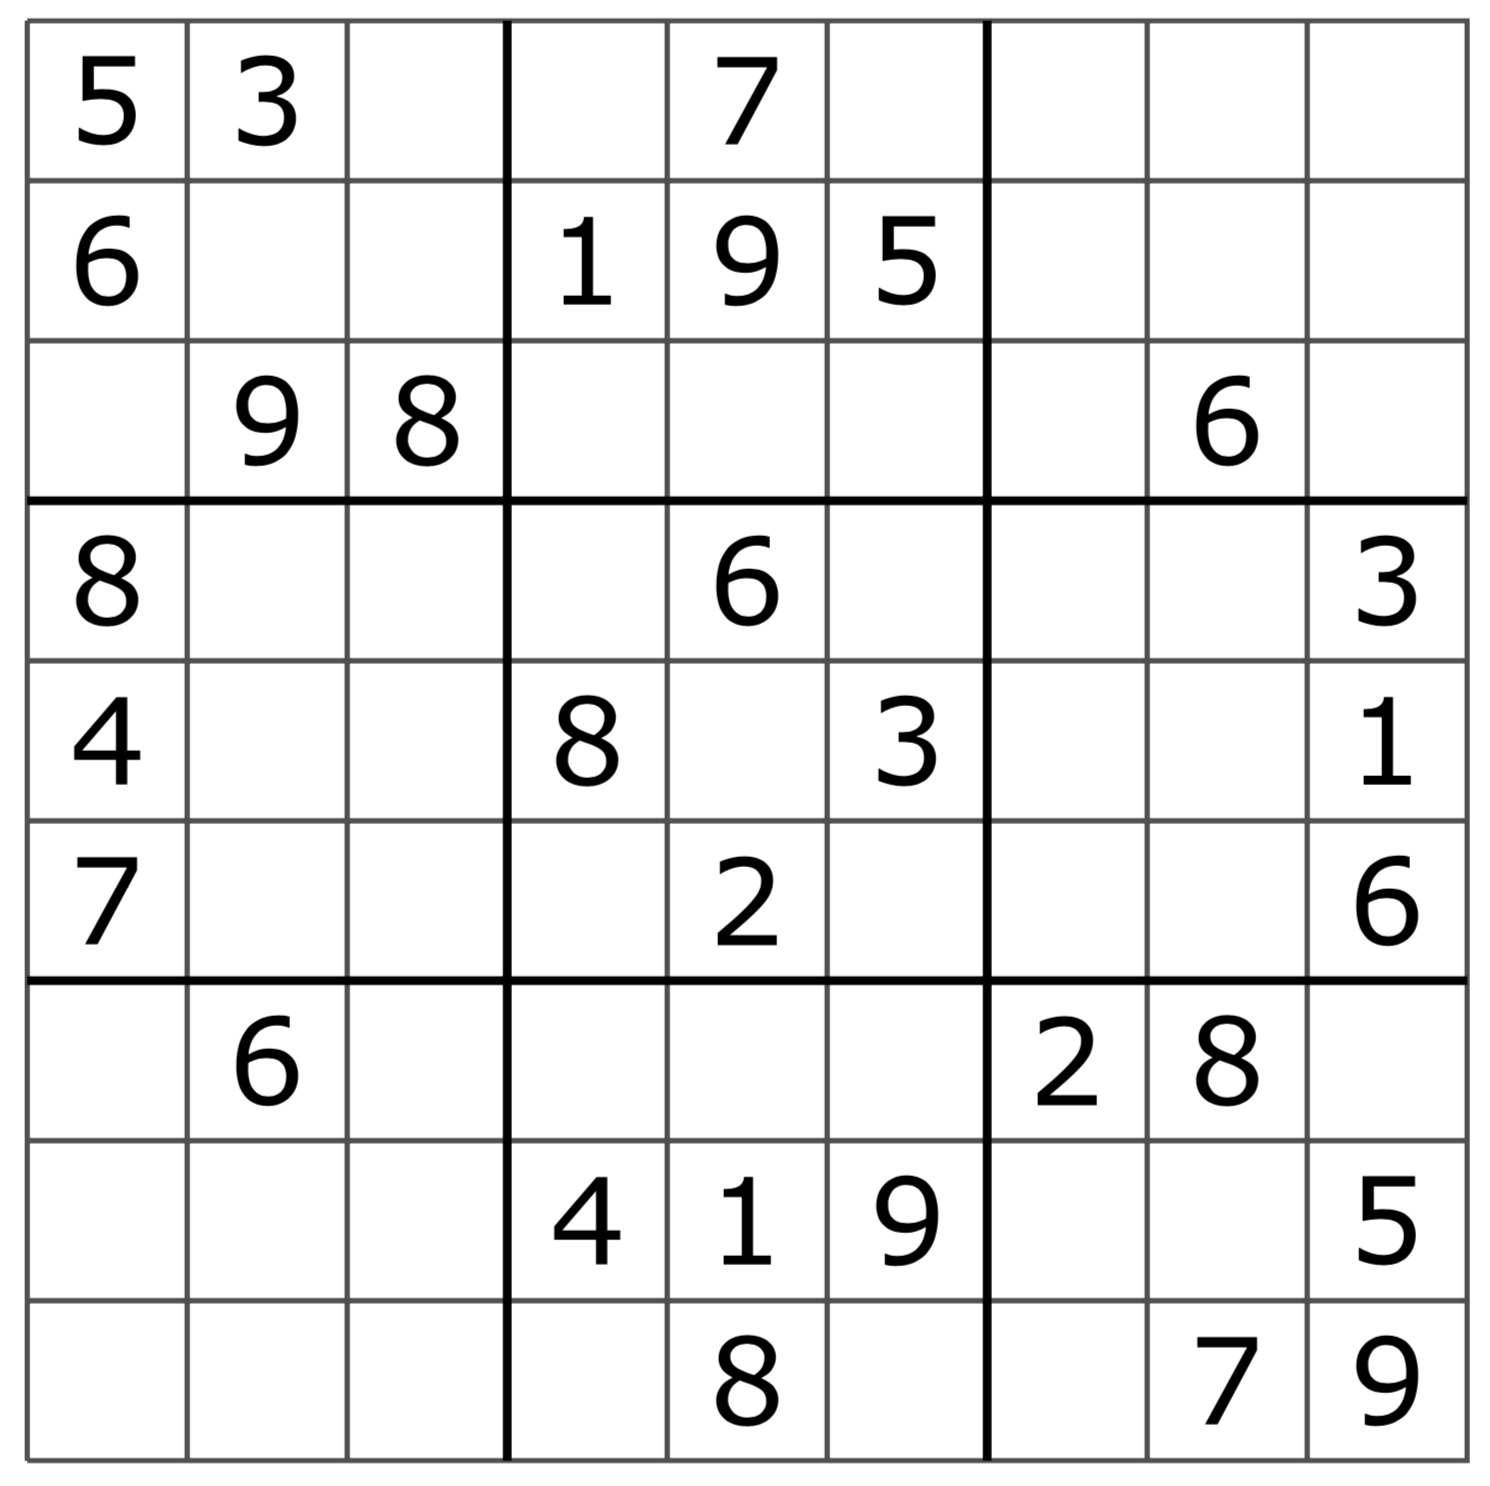
\includegraphics[width=70mm]{assets/sudoku.png}
\end{frame}

\begin{frame}
\frametitle{Persistent storage with files.}

\begin{itemize}
\item \emc{File systems} provide persistent storage, and expose it through a hierarchy of \emc{directories} and \emc{files}.
\item A file is a \emc{sequence of bytes} written to persistent memory (disk or other).
\item Files support \emc{read} and \emc{write} operations on arbitrary positions of this sequence, as well as \emc{updating} and \emc{appending} data at the end of files.
\end{itemize}

Python supports handling files in \texttt{text mode} or \texttt{binary mode}. The first takes care of encoding of stings semi-automatically, while the second is more flexible but requires manual conversion of everything to bytes.

\end{frame}

\begin{frame}
\frametitle{The open function.}

The \texttt{open} function takes as parameters a file path and a mode, and returns a file object that may be used to \texttt{read} or \texttt{write}. All files should be \emc{closed} after processing.

\vspace{3mm}
Modes include a combination of text (`t') or binary (`b'); read (`r'), write and truncate (`w') or append (`a'); and optionally update (`+').

\vspace{3mm}
The full documentation for \texttt{open}: \url{https://docs.python.org/3/library/functions.html\#open}

\end{frame}

\begin{frame}
\frametitle{Reading all data from a text file.}

	\inputminted[
		firstline=3,
		lastline=7,
		xleftmargin=1.4em,
		frame=lines,
		framesep=2mm,
		fontsize=\footnotesize,
		linenos
	]{python}{src/open.py}

Calling \texttt{read()} reads the full contents of the file into memory. Remember to \emc{close files} to free system resources.


\end{frame}

\begin{frame}
\frametitle{Reading and writing text files.}

	\inputminted[
		firstline=11,
		lastline=20,
		xleftmargin=1.4em,
		frame=lines,
		framesep=2mm,
		fontsize=\footnotesize,
		linenos
	]{python}{src/open.py}

\begin{itemize}
	\item Opening a file with `w' \emc{truncates} the file. (`r+' to update; `a' to append.)
	\item A file is an \emc{iterator}. The \texttt{for} loop reads each line in turn.
	\item Closing files can get tedious.
\end{itemize}


\end{frame}

\begin{frame}
\frametitle{The `with' control structure.}

\emc{Acquiring and freeing} resources is a very common pattern. The with control structure removes the need for manual closing of files, or freeing resources.

	\inputminted[
		firstline=22,
		lastline=29,
		xleftmargin=1.4em,
		frame=lines,
		framesep=2mm,
		fontsize=\footnotesize,
		linenos
	]{python}{src/open.py}

\end{frame}

\begin{frame}
\frametitle{Working with binary files.}

You can use \emc{seek} and \emc{tell} to select a position in the file. 
	\inputminted[
		firstline=31,
		lastline=39,
		xleftmargin=1.4em,
		frame=lines,
		framesep=2mm,
		fontsize=\footnotesize,
		linenos
	]{python}{src/open.py}


\end{frame}

\begin{frame}[fragile]
\frametitle{Standard input and output.}

Programs have a standard input and standard output that act as files for reading and writing data.

	\inputminted[
		firstline=43,
		lastline=47,
		xleftmargin=1.4em,
		frame=lines,
		framesep=2mm,
		fontsize=\footnotesize,
		linenos
	]{python}{src/open.py}

	\inputminted[
		firstline=58,
		lastline=59,
		xleftmargin=1.4em,
		frame=lines,
		framesep=2mm,
		fontsize=\footnotesize,
		linenos
	]{python}{src/open.py}


\begin{Verbatim}
$ echo "Hello" | python src/open.py
HELLO
\end{Verbatim}

\end{frame}


\begin{frame}
\frametitle{How to test programs that access the environment.}

`\emc{Monkeypatching}' is a test tactic in which you \emc{substitute functions that access the environment} with known `dummy' ones.

	\inputminted[
		firstline=49,
		lastline=56,
		xleftmargin=1.4em,
		frame=lines,
		framesep=2mm,
		fontsize=\footnotesize,
		linenos
	]{python}{src/open.py}

You can monkey patch to \emc{inject known data} pretending to be the environment. Or to \emc{test interactions} with the environment. Tests should not access the environment.

\end{frame}


\begin{frame}
\frametitle{Dealing with a lot of data.}

\emc{Big data}: Some processing tasks involve datasets that are \emc{larger than the working memory} of a single computer.
\begin{itemize}
\item Reading the full file in memory is not possible.
\item Instead \emc{on-line algorithms} must be implemented to \emc{work incrementally}.
\item Read small chunks of data; process; write small chunks of output.
\end{itemize}

\begin{block}{Sorting files on disk}
Early computers had a tiny amount of working memory, and used tapes as persistent storage. Mergesort was especially important since it may be used to sort files in an incremental way with access to very little memory.
\end{block}

\end{frame}

\begin{frame}
\frametitle{The social importance of sorting and indexing.}

Modern search engines, need to find information within milliseconds!

\vspace{3mm}
Fast information retrieval is achieved through \emc{indexing}:
\begin{itemize}
	\item The file to be indexed is scanned linearly, and a list of tuples of (word, byte position) are extracted.
	\item The tuples are then sorted to produce an \emc{inverted index}.
	\item The inverted index is stored to disk alongside the file.
	\item To find all instances of a term binary search is used on the inverted index to \emc{retrieve the positions} in the file, if any, the term appears.
\end{itemize}

The second ingredient of search engines is \emc{ranking}, that selects which files are most relevant for a search term.
\end{frame}

\begin{frame}
\frametitle{Searching, Indexing, Files \& Privacy.}

Data have \emc{meaning}, and can impact people's lives.\\
Protecting \emc{people's rights}, including \emc{privacy}, part of professional conduct.

\vspace{3mm}
UK Data Protection Act and the new General Data Protection Regulations:
\begin{itemize}
	\item Defines `personal information' as anything relating to a living individual.
	\item Lawful grounds (consent, contract, law) must exist to process.
	\item Can only store for defined purposes, time frames.
	\item Must be secured.
	\item Rights: access, remedy, to be forgotten.
\end{itemize}

{\small \url{https://ico.org.uk/for-organisations/guide-to-data-protection/}}

\end{frame}


\begin{frame}
\frametitle{Technical implications of regulations.}

\begin{itemize}
	\item All personal information is mutable.
	\item Need to be able to find and remove it \\ (Right to be Forgotten, Subject Access).
	\item That includes indexes and file backups.
	\item Notices and privacy statements need to be provided.
	\item No data processing should take place beyond what was notified.
	\item You need to use appropriate security controls.
\end{itemize}

\end{frame}


\bibliographystyle{alpha}
\nobibliography{references}

\end{document}
